\renewcommand{\FileName}{heplot2}
% slide template
\begin{frame}
  \frametitle{HE plots: Visualization for the MLM}
  \begin{itemize}
	\item{\large\bfseries LM}: $\vec{y} = \mat{X} \vec{\beta} + \vec{\epsilon}$
      \begin{itemize*}
	  \item Test \emph{any} hypothesis by \emph{General Linear Test}: $H_0 : \mat{C} \vec{\beta} = \vec{0}$,
	  where $\mat{C}= $ matrix of constants; rows specify $h$ linear combinations or contrasts of parameters.
	  \item e.g., Test of $H_0 : \beta_1 = \beta_2 = 0$ in model $y_i = \beta_0 + \beta_1 x_{1i} + \beta_2 x_{2i} + \epsilon_i$
	\begin{equation*}
	\mat{C} \vec{\beta} = \left[
	\begin{array}{rrr}
    0  &  1  &  0 \\
	0  &  0  &  1
	\end{array}\right]
	\left(
	\begin{array}{l}
	\beta_0 \\ \beta_1 \\ \beta_2
	\end{array}
	\right)
	=
	\left(
	\begin{array}{l}
	0 \\ 0
	\end{array}
	\right)
	\end{equation*}
	  \item All $\rightarrow$ F-test:  How big is $SS_H$ relative to $SS_E$?
	\begin{equation*}
F = \frac{SS_H / \textrm{df}_h}{SS_E / \textrm{df}_e} = \frac{MS_H}{MS_E} \longrightarrow
  ( MS_H - F \: MS_E ) = 0
	\end{equation*}
	  \end{itemize*}

\end{frame}

\begin{frame}
  \frametitle{HE plots: Visualization for the MLM}
	\item{\large\bfseries MLM}: $\mat{Y} = \mat{X} \vec{B} + \mat{E}$, for $p$ responses, $\mat{Y} = (\vec{y}_1 , \vec{y}_2, \dots , \vec{y}_p )$
      \begin{itemize*}
	  \item \emph{General Linear Test}: $H_0 : \mat{C} \vec{B} = \mat{0}$
	  \item Analogs of sums of squares, $SS_H$ and $SS_E$ are $(p \times p)$ matrices, \H and \E,
\begin{equation*}% \label{eq:hmat}
\mat{H}  =
 (\mat{C} \widehat{\mat{B}})\trans \,
 [\mat{C} (\mat{X}\trans \mat{X} )^{-} \mat{C}\trans]^{-1} \,
 (\mat{C} \widehat{\mat{B}})
 \comma
\end{equation*}
\begin{equation*}% \label{eq:emat}
\mat{E}  =
 \mat{Y}\trans
 [\mat{I} - \mat{H}]
 \mat{Y}
 \period
\end{equation*}
	\item Analog of univariate $F$ is
\begin{equation*}%\label{eq:mtest1}
 | \mat{H} - \lambda \mat{E} | = 0
 \comma
\end{equation*}
	\item How big is \H relative to \E ?
	\begin{itemize*}
	\item Latent roots $\lambda_1 , \lambda_2, \dots \lambda_s$ measure the ``size'' of \H relative to \E{} in $s=\min(p, df_h)$
	orthogonal directions.
	\item Test statistics (Wilks' $\Lambda$, Pillai trace criterion, Hotelling-Lawley trace criterion, Roy's maximum root)
	all combine info across these dimensions
	\end{itemize*}
	\item HE plot:  Shows size, dimensionality, and effect-correlation of \H relative to \E{}.
	  \end{itemize*}
  \end{itemize}
\end{frame}

  \begin{frame}
	\frametitle{Didactic displays for MANOVA tests}

  \begin{center}
	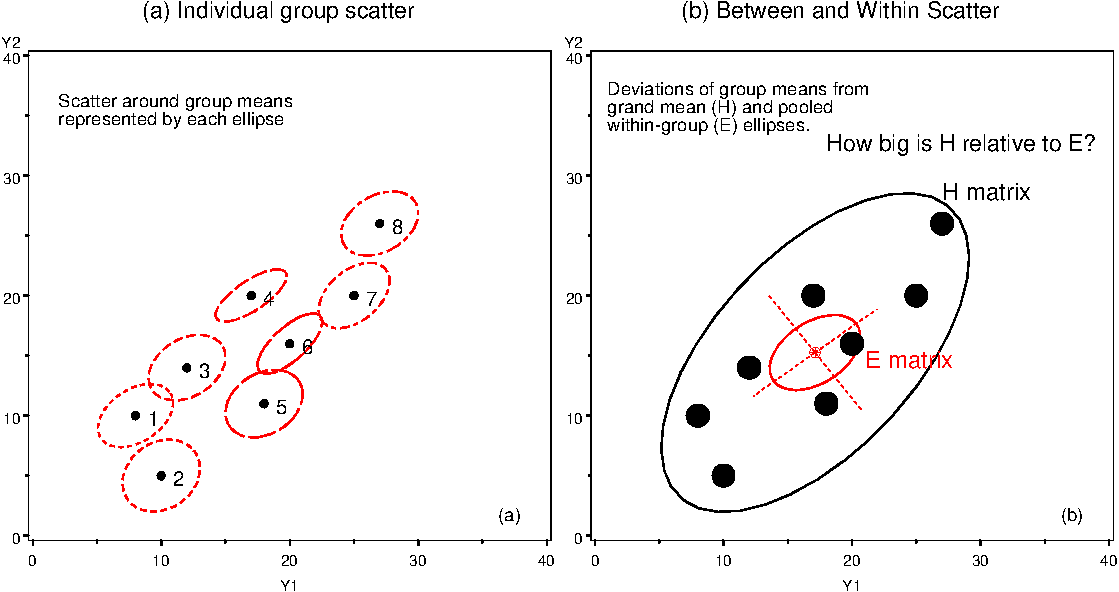
\includegraphics[width=.9\textwidth,clip]{fig/arcmanov1}
	\\ Essential ideas behind multivariate tests: (a) Data ellipses; (b) \H and \E matrices
  \end{center}

  \begin{center}
	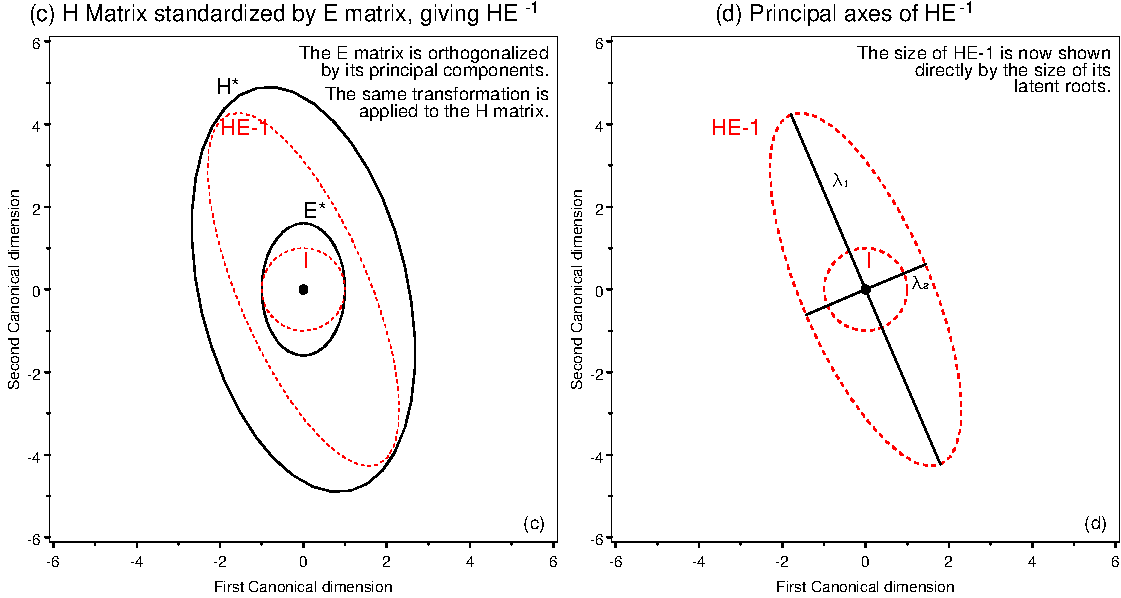
\includegraphics[width=.9\textwidth,clip]{fig/arcmanov2}
	\\ Essential ideas behind multivariate tests: latent roots of $\mat{H} \mat{E}^{-1}$
  \end{center}
  \end{frame}

  \begin{frame}
	\frametitle{HE plot for iris data}

  \begin{center}
	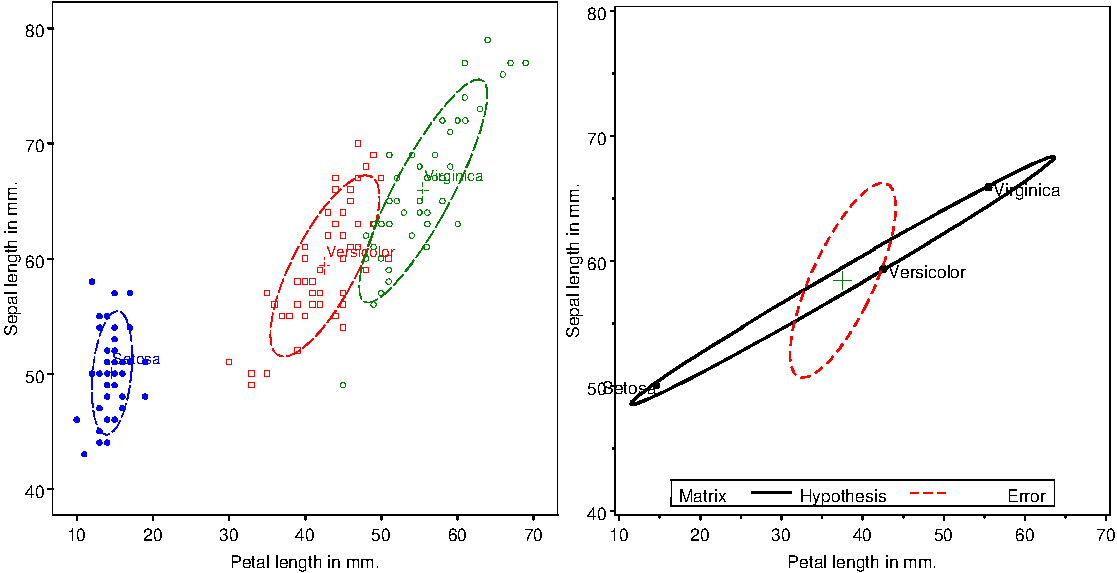
\includegraphics[width=.9\textwidth,clip]{fig/heplot31}
	\\ (a) Data ellipses and (b) \H and \E matrices (scaled by $1/df_e$: effect size)
%	\\ NB: Plotting $\sqrt{n} \mat{H} / dfe$:  shows evidence against $H_0$ in the sample
  \end{center}
  \begin{itemize*}
  	\item \mat{H} ellipse:  data ellipse for fitted values, $\hat{\vec{y}}_{ij} =
	\bar{\vec{y}}_j$.
	\item \mat{E} ellipse:  data ellipse of residuals, $\hat{\vec{y}}_{ij} -
	\bar{\vec{y}}_j$.
  \end{itemize*}
  \end{frame}



